\documentclass[tikz,border=8pt]{standalone}
% Shared look for every TikZ diagram. Load with \input{../../tools/tikz-style.tex}
\usepackage[T1]{fontenc}
\usepackage{lmodern}
\renewcommand{\sfdefault}{lmr}  % diagrams use the same serif as the text
\usetikzlibrary{arrows.meta, positioning, shapes.geometric, calc, fit, backgrounds}
\definecolor{cblue}{HTML}{4C78A8}
\definecolor{corange}{HTML}{F58518}
\definecolor{cgreen}{HTML}{54A24B}
\definecolor{cred}{HTML}{E45756}
\definecolor{cpurple}{HTML}{B279A2}
\definecolor{cgrey}{HTML}{6B6B6B}
\tikzset{
  every picture/.style={font=\sffamily, line width=1.2pt},
  box/.style={draw=#1, fill=#1!12, rounded corners=4pt, align=center, inner sep=7pt, minimum height=1.1cm},
  box/.default=cgrey,
  arrow/.style={-{Stealth[length=3mm]}, draw=cgrey, line width=1.4pt},
  title/.style={font=\sffamily\bfseries\Large},
  note/.style={font=\sffamily\small, text=cgrey, align=center},
}
\AtBeginDocument{\hyphenpenalty=10000 \exhyphenpenalty=10000}

% scale: 1 data unit = 5 cm.  u = [0.6, 0.8], i = [1, 0]
\begin{document}
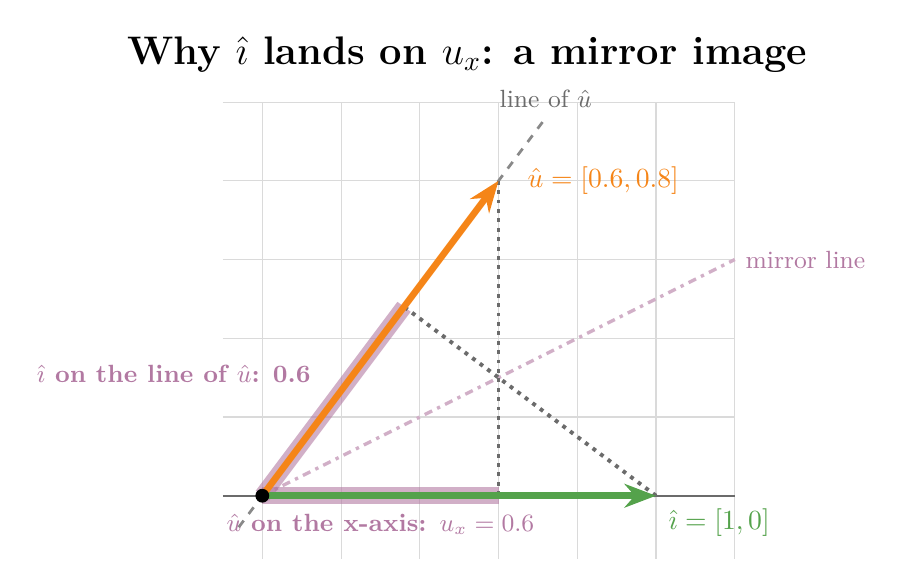
\begin{tikzpicture}
  \node[title] at (2.6,5.6) {Why $\hat{\imath}$ lands on $u_x$: a mirror image};
  \draw[cgrey!25, line width=0.4pt] (-0.5,-0.8) grid (6,5);
  \draw[cgrey, line width=0.8pt] (-0.5,0) -- (6,0);
  \draw[cgrey!80, dashed, line width=1pt] (-0.3,-0.4) -- (3.6,4.8) node[above, note] {line of $\hat{u}$};
  \draw[cpurple!60, dash dot, line width=1.2pt] (0,0) -- (6,3) node[right, note, text=cpurple] {mirror line};
  % the two shadows, each of length 0.6
  \draw[cpurple, line width=6pt, opacity=0.6] (0,0) -- (3,0);
  \draw[cpurple, line width=6pt, opacity=0.6] (0,0) -- (1.8,2.4);
  \draw[cgrey, dotted, line width=1.4pt] (3,4) -- (3,0);
  \draw[cgrey, dotted, line width=1.4pt] (5,0) -- (1.8,2.4);
  \draw[-{Stealth[length=4mm]}, cgreen, line width=2.4pt] (0,0) -- (5,0) node[below right, font=\bfseries] {$\hat{\imath} = [1, 0]$};
  \draw[-{Stealth[length=4mm]}, corange, line width=2.4pt] (0,0) -- (3,4) node[right, xshift=6pt, font=\bfseries] {$\hat{u} = [0.6, 0.8]$};
  \node[font=\small\bfseries, text=cpurple, below] at (1.5,-0.1) {$\hat{u}$ on the x-axis: $u_x = 0.6$};
  \node[font=\small\bfseries, text=cpurple, anchor=east] at (0.75,1.55) {$\hat{\imath}$ on the line of $\hat{u}$: 0.6};
  \fill (0,0) circle (2.5pt);
\end{tikzpicture}
\end{document}
